\begin{figure*}[t]
    \centering
    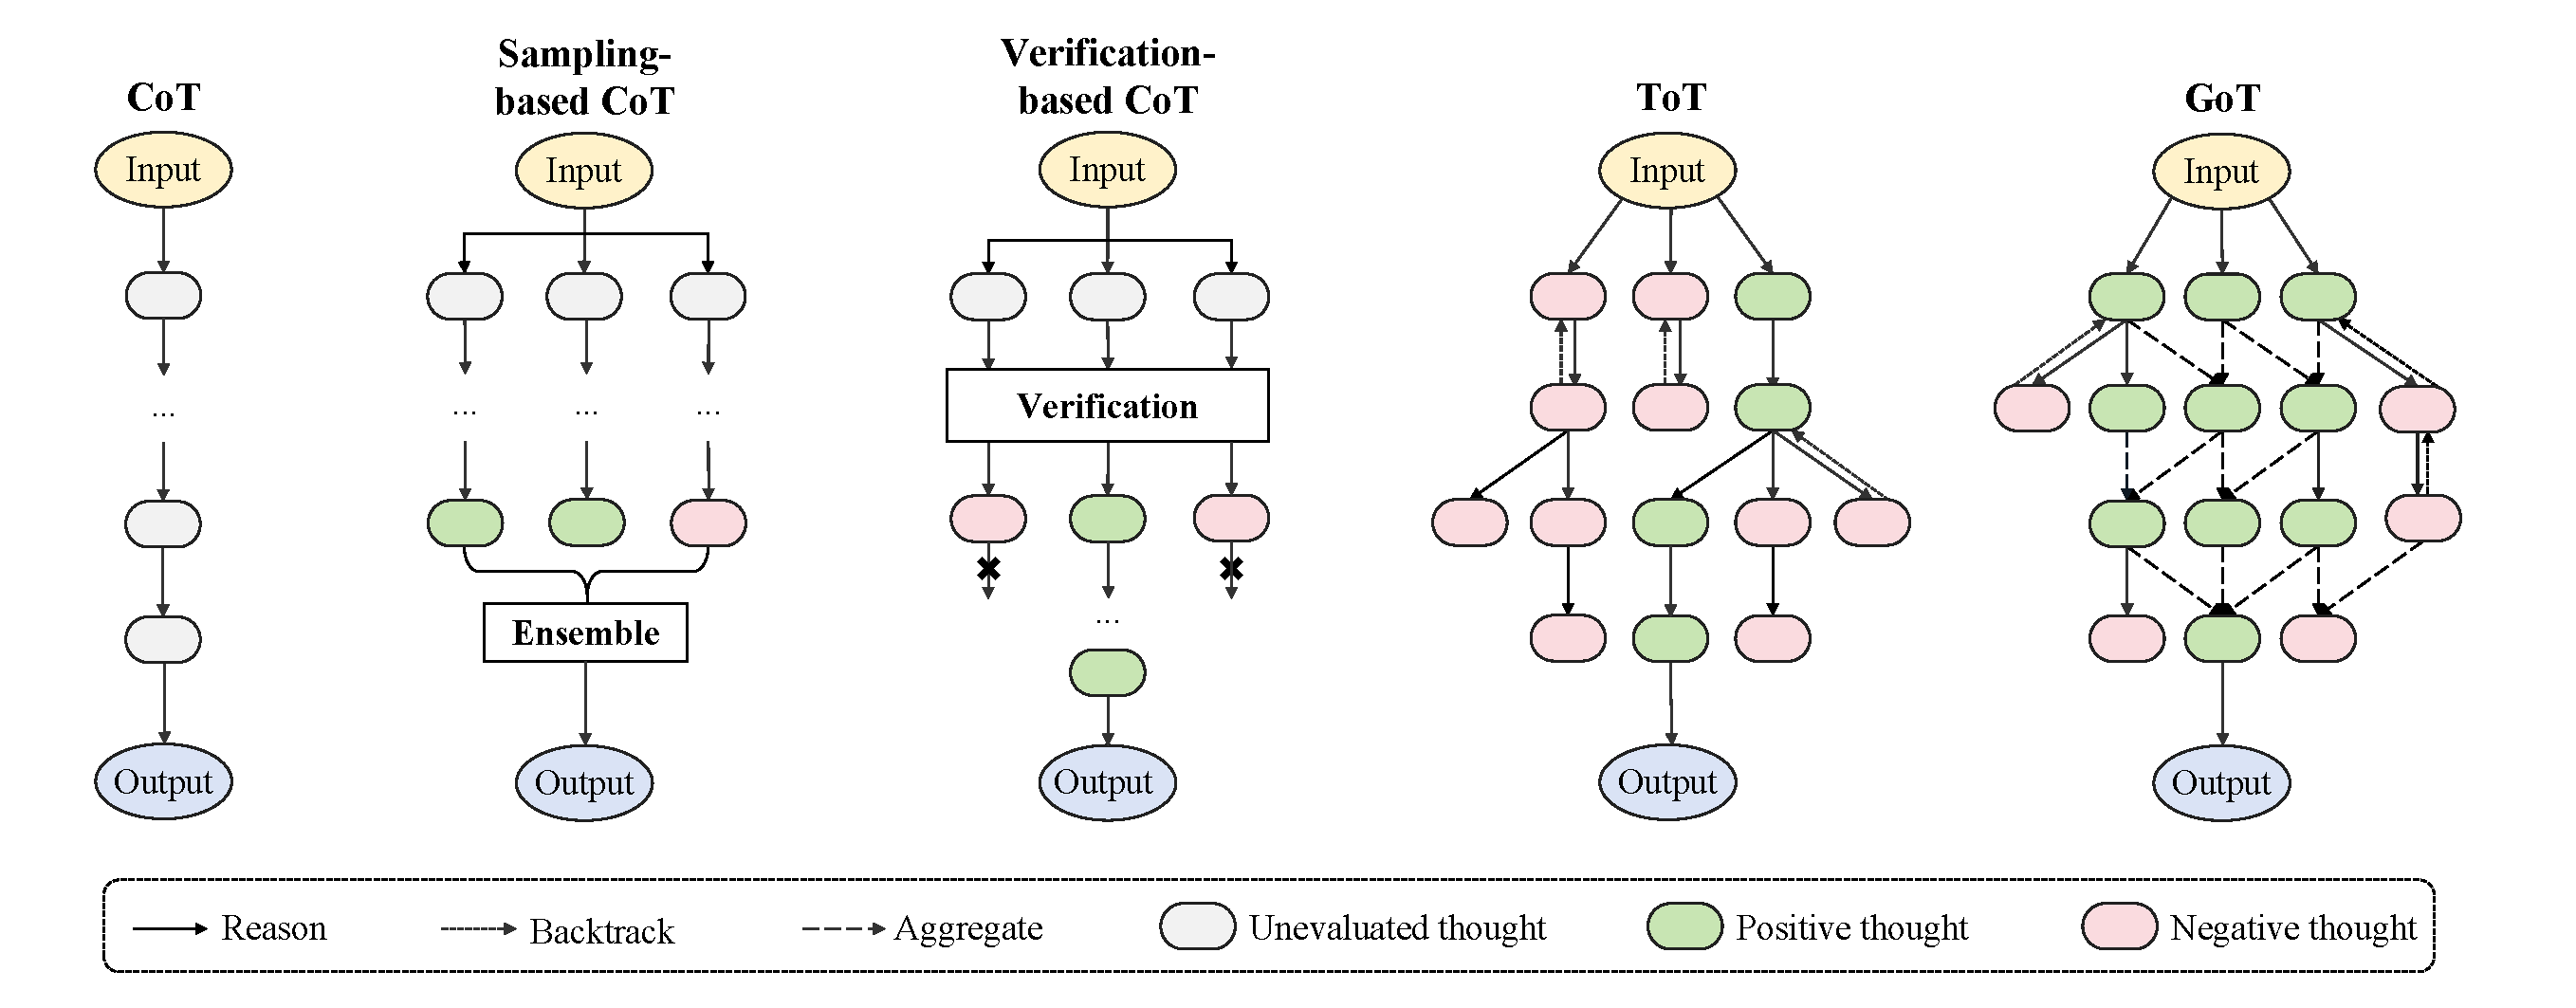
\includegraphics[width=\textwidth]{images/XoT.pdf}
    \caption{
        An illustration of the evolution of CoT prompting strategies. It begins with the basic CoT approach and progresses to enhanced CoT generation techniques,  including sampling-based and verification-based methods. Finally, it extends to variations of the chain structure, such as trees and graphs. Here, ``thought'' refers to an intermediate reasoning step as stated in~\cite{Wei-arxiv-2022-chain, Yao-arxiv-2023-Tree}.
    }
\label{fig:extension_of_CoT}
\end{figure*}

\subsection{Chain-of-Thought Prompting}
\label{subsec-cot}

Chain-of-Thought~(CoT) prompting~\cite{Wei-arxiv-2022-chain, Chu-arxiv-2023-A} is an improved prompting strategy to boost the performance of LLMs on complex reasoning tasks, such as arithmetic reasoning~\cite{Miao-ACL-2020-A}, commonsense reasoning~\cite{Talmor-naacl-2019-CommonsenseQA}, and symbolic reasoning~\cite{Wei-arxiv-2022-chain}.
Instead of simply constructing the prompts with input-output pairs like ICL, CoT prompting further incorporates intermediate reasoning steps, which serve as the bridge between inputs and outputs.
{
Figure~\ref{fig:utilization} presents an illustration of CoT.
In the following part, we will first elaborate on the basic CoT prompting approach and its improved strategies, then discuss when and why CoT prompting works.
}

\subsubsection{Basic CoT Prompting Approach}


{
}

CoT prompting is first proposed as an extension of ICL~\cite{Wei-arxiv-2022-chain}, which augments each demonstration $\langle$\emph{input, output}$\rangle$ as $\langle$\emph{input, CoT, output}$\rangle$.
A \textit{CoT} is a series of intermediate reasoning steps for connecting the \textit{input} and \textit{output}.
With these augmented demonstrations, LLMs can follow them to  %
{generate CoTs and the answer for a new input.} 
However, unlike $\langle$\emph{input, output}$\rangle$ pairs in ICL, CoTs are difficult to obtain and usually require human annotation.
Fortunately, it has been found that LLMs can be triggered to generate CoTs through simple instructions like ``\emph{Let's think step by step.}''~\cite{Kojima-arxiv-2022-Large}, making CoT prompting easy to use.
There are also alternative magic prompts that {can elicit the ability of CoT reasoning and further improve the performance of LLMs}, such as ``\emph{Take a deep breath and work on this problem step-by-step.}''~\cite{Yang-CoRR-2023-Large}.

{
As illustrated in Figure~\ref{fig:extension_of_CoT}, the generation process of CoT follows a chain structure in the basic CoT prompting approach, where LLMs generate CoTs step by step.
Typically, CoT takes the format of natural language text.
However, textual CoTs may not work well on complex tasks that require rigorous logic for reasoning.
Considering this, some work uses code~\cite{Chen-arxiv-2022-Program, Gao-ICML-2023-PAL} due to its structured and precise nature.
Furthermore, the authors in~\cite{Zhao-arxiv-2023-Automatic} propose to dynamically select text or code as the format of CoTs to combine their advantages.
}





\subsubsection{Improved CoT Prompting Strategies}

{
Despite the performance improvement in complex reasoning tasks, CoT prompting still suffers from problems like incorrect reasoning and instability.
In this part, we first introduce how to design better CoT prompts and enhanced CoT generation strategies, and then introduce the extension of the basic chain structure of CoT.
Figure~\ref{fig:extension_of_CoT} illustrates the evolution of representative CoT prompting strategies.
}

\paratitle{Better Prompt Design.}
Since CoT prompting relies on prompts to elicit the reasoning capabilities of LLMs, the design of prompts is critical to its performance.
As a direct approach, it is shown that using diverse CoTs (\ie multiple reasoning paths for each problem) can effectively enhance the performance~\cite{Li-arxiv-2022-On}.
Another intuitive idea is that prompts with more complex reasoning paths are more likely to elicit the reasoning ability of LLMs~\cite{Fu-arxiv-2022-Complexity}, which can result in higher accuracy in generating correct answers.
However, all these approaches rely on annotated CoT datasets, which limits their use in practice. 
To overcome this limitation, magic instructions such as  ``\emph{Let's think step by step}'' can be used to automatically construct CoTs by prompting LLMs~\cite{Zhang-arxiv-2022-Automatic}. 


\paratitle{Enhanced CoT Generation.}
{
Since LLMs are prone to producing incorrect reasoning steps and exhibiting instability in the generation process, there are a number of studies~\cite{Li-arxiv-2023-Making, Wang-arxiv-2022-Self-Consistency} to improve the generation of CoT.
In this part, we will introduce two typical approaches to enhancing the generation of CoT: sampling- and verification-based methods.
}

$\bullet$ \emph{Sampling-based methods.}
{
LLMs are known to suffer from instability during inference, which can lead to unfaithfulness in the generated reasoning steps.
To address this issue, some work proposes to sample multiple reasoning paths instead of using greedy decoding.
As a representative solution, self-consistency~\cite{Wang-arxiv-2022-Self-Consistency} 
first generates several reasoning paths and then takes an ensemble over the corresponding answers,  selecting the most consistent one through majority voting.
However, such a method can still lead to wrong answers when most of the reasoning paths are misled.
Considering this, the authors in~\cite{Fu-arxiv-2022-Complexity} only vote on the $k$ most complex reasoning paths based on their observation that reasoning paths with higher complexity (\eg more reasoning steps) usually have better performance. 
{Furthermore, MCR~\cite{Yoran-arxiv-2023-Answering} proposes referring to the steps from other reasoning paths when generating the next step, and performs reasoning across multiple reasoning paths to generate the final answer.}
}

$\bullet$ \emph{Verification-based methods.} {
The sequential nature of reasoning steps in CoTs can lead to the accumulation of errors in the generated CoTs when certain steps are incorrect. 
To mitigate this problem, recent studies propose to verify the correctness of generated reasoning steps with either trained verifiers or LLMs themselves. 
For example, DIVERSE~\cite{Li-arxiv-2023-Making} trains solution-level and step-level verifiers respectively to examine the reasoning steps at different granularities. 
Another approach~\cite{Ling-arxiv-2023-Deductive} utilizes LLMs to verify the correctness of reasoning steps through step-by-step self-verification with a specially designed reasoning format.
In addition, several studies propose backward reasoning for verification: 
it first deduces the necessary question conditions~\cite{Xue-arxiv-2023-RCOT, Weng-arxiv-2023-Large} or variables~\cite{Jiang-arxiv-2023-Forward} {from the model's predictions}, and then compares them with the original ones.
}

\paratitle{Reasoning Structure Extension.}   
{
Despite the generality, the chain reasoning structure of basic CoT prompting limits its effectiveness in solving complex tasks, which require exploration like foresight and backtracking during inference.
Therefore, many studies have been devoted to extending the reasoning structure by designing more intricate thought processes, \eg tree- and graph-structured reasoning. %
}

$\bullet$ \emph{Tree-structured reasoning.} 
This approach (exemplified by Tree of Thoughts~(ToT)~\cite{Yao-arxiv-2023-Tree, Long-arxiv-2023-Large}) formulates the reasoning process in a hierarchical tree structure, where intermediate thoughts are nodes.
{In this way, it enables  LLMs to explore multiple reasoning paths in parallel and further supports the operation of lookahead and backtracking to facilitate more comprehensive decisions.} 
In addition, TouT~\cite{Mo-arxiv-2023-Tree} takes the uncertainty of intermediate thoughts into account for thought evaluation based on Monte Carlo Dropout.

$\bullet$ \emph{Graph-structured reasoning.} {
Although the tree structure facilitates parallel reasoning, it also imposes restrictions on the reasoning process.
With more complex topological structures, graphs offer greater flexibility in reasoning, enabling the characterization of more intricate relationships and interactions.
For instance, Graph of Thoughts~(GoT)~\cite{Besta-arxiv-2023-Graph, Lei-arxiv-2023-Boosting} conceptualizes the reasoning process as an arbitrary graph, where vertices denote intermediate thoughts and edges denote the interdependence between these thoughts. 
{Compared with ToT, it can further utilize thoughts from other reasoning paths when generating new thoughts.}
However, such an approach requires a large number of interactions with LLMs, making the thought exploration process highly inefficient. 
} 
{
To reduce potentially meaningless thought exploration, XoT~\cite{ding-arxiv-2023-everything} further proposes to guide the search of thoughts with pre-trained policy and value networks.
}





\subsubsection{Further Discussion on CoT Prompting}
In this part, we present discussions regarding two fundamental questions related to CoT prompting, \ie ``\textit{when does CoT prompting work for LLMs}'' and ``\textit{why can LLMs perform CoT reasoning}''.

\paratitle{{When CoT Prompting Works For LLMs?}} 
Since CoT reasoning is an emergent ability~\cite{Wei-arxiv-2022-Emergent}, it only has a positive effect on sufficiently large models (typically containing 10B or more parameters~\cite{Wei-arxiv-2022-chain}) but not on small models. 
Moreover, since CoT prompting augments the standard prompting with intermediate reasoning steps, it is mainly effective for the tasks that require step-by-step reasoning~\cite{Wei-arxiv-2022-chain}, \eg arithmetic reasoning, commonsense reasoning, and symbolic reasoning.
Whereas, for other tasks that do not rely on complex reasoning, CoT prompting might lead to worse performance than standard prompting~\cite{Wang-arxiv-2022-Rationale}, \eg MNLI-m/mm, SST-2, and QQP from GLUE~\cite{Wang-EMNLP-2018-GLUE}.   
Interestingly, it seems that the performance gain brought by CoT prompting could be significant only when standard prompting yields poor results~\cite{Wei-arxiv-2022-chain}.

\paratitle{{Why LLMs Can Perform CoT Reasoning?}} 
As the second question, we discuss the underlying mechanism of CoT prompting in the following two aspects. 

$\bullet$ \emph{The source of CoT reasoning ability}. 
Regarding the source of CoT reasoning capability, it is widely hypothesized that it can be attributed to training on code since models trained on it show a strong reasoning ability~\cite{Liang-arxiv-2022-Holistic, FU-blog-2022-how, Bi-arxiv-2023-When}.   
Intuitively, code data is well organized with algorithmic logic and programming flow, which may be useful to improve the reasoning performance of LLMs. 
However, this hypothesis still lacks publicly reported evidence of ablation experiments (\emph{with} and \emph{without} training on code). 
In addition, instruction tuning seems not to be the key reason for obtaining the CoT reasoning ability, since 
it has been empirically shown that instruction tuning on non-CoT data does not improve the performance on held-out CoT reasoning benchmarks~\cite{Chung-arxiv-2022-Scaling}.

$\bullet$ \emph{The effect of CoT prompting components}. 
The major distinction between CoT prompting and standard prompting is the incorporation of reasoning paths prior to the final answer. 
Thus, some researchers investigate the effects of different components in the reasoning paths. 
Specifically, a recent study identifies three key components in CoT prompting, namely  \emph{symbols}~(\eg numerical quantities in arithmetic reasoning), \emph{patterns}~(\eg equations in arithmetic reasoning), and \emph{text}~(\ie the rest of tokens that are not symbols or patterns)~\cite{Madaan-arxiv-2022-Text}. 
It is shown that the latter two parts (\ie patterns and text) are essential to the model performance, and removing either one would lead to a significant performance drop. 
However, the correctness of symbols and patterns does not seem critical. 
Further, there exists a symbiotic relationship between text and patterns:   the text helps LLMs to generate useful patterns, and patterns aid LLMs to understand tasks and generate texts that help solve them~\cite{Madaan-arxiv-2022-Text}.


In summary, CoT prompting provides a general and flexible approach to eliciting the reasoning ability of LLMs. 
There are also some preliminary attempts to extend this technique to solve multimodal~\cite{Zhang-arxiv-2022-Multimodal} and multilingual tasks~\cite{Shi-arxiv-2022-Language}.